%%%%%%%%%%%%%%%%%%%%%%%%%%%%%%%%%%%%%%%%%%%%%%%%%%%%%%%%%%%%%%%%%%%%
% Technologies and Implementation
%%%%%%%%%%%%%%%%%%%%%%%%%%%%%%%%%%%%%%%%%%%%%%%%%%%%%%%%%%%%%%%%%%%%

\chapter{Implementation}
  \label{Implementation}
The following chapter explains how the user interface is structured and which options the user is given to ... after describing the intent of this project.
\section{Motivation and intent}
As mentioned in the introduction, figuring out a linear layout with certain properties by hand is a time consuming, error-prone task which is why the desire for automation is a understandable one.\\
The discovery that SAT formulas could do this quite efficiently\cite{Bekos2015TheBE} was a big achievement and the logical next step was finding a way to create specific graphs in a visually appealing and well structured way. \\
Furthermore it was an ambition to check a graph for specific linear layouts, since randomized SAT-sovers produce random linear layouts. Thankfully this  can be achieved by expanding the formula by clauses that lead the SAT-solver in the desired direction. Therefore adding the means to impose such constraints upon a linear layout was the second big part of this project.
\section{Graph Editor}
\begin{figure}[!h]
\begin{center}

\includegraphics[width=1\textwidth]{figures/Platzhalter.png}
\caption{Overview over the user interface}
\label{img:overviewIndex}
\end{center}
\end{figure}
\subsection{Overwiew}
The user interface of this tool consists of three main areas: the toolbar on top, the interactive graph editor in the middle and the bottom part, where the user can specify the linear layout he wishes to compute.\\
\subsection{Graph Editor}
The main component, the graph editor is the center area of the user interface. It displays a grid by default which can be disabled in the \textit{view} submenu.\\
\subsubsection{User Interaction}
By double-clicking the user can create nodes on the canvas. An edge is created by clicking and dragging on a node that is not selected, releasing either when another node is reached or if the user wants to create a bend, releasing wherever the bend should be. Note that duplicate edges are forbidden in this environment. \\
The user can also select several or all elements of the graph and move them on the canvas. The elements will propose positions by clipping to the grid but can be placed freely. The clipping is disabled when the grid is hidden.\\
All elements of the graph can be deleted, copied, cut and pasted. 
By right clicking on one or more nodes or edges, a context menu opens and displays a selection of constraints that can be imposed on the to be calculated linear layout. The different kinds of constraints are described in the corresponding section.
\subsubsection{Identifier of elements}
To compute the linear layout of the graph it is necessary to have a unique id for each element of the graph, so the solver can distinguish the different nodes and edges.\\
On creation every node and edge is assigned a label, which is displayed in the graph editor and can be changed by the user without restriction. Invisible for the user each node and edge also is assigned a tag, a feature provided by the \textit{yFiles for HTMl} library. These tags can not be changed by the user and are designed to be unique. Nodes simply get the next free number as a tag, edges get the tag "a-b", where a is the tag of the source node and b is the tag of the target node. These unique tags are what is used in the solving process.\\
\subsection{Toolbar}
On the left section of the toolbar the user can choose from submenus similar to most editors, the options being a \textit{file}, \textit{edit}, \textit{view}, \textit{layout} as well as a link to the about information of this page and a button to toggle the visibility of \textcolor{red}{the bottom part of the page.}.\\
\begin{figure}[!h]
\begin{center}

\includegraphics[scale=0.5]{figures/figIndex/FileToolbar.jpg}
\caption{Contents of the \textit{file} submenu}
\label{img:fileToolbar}
\end{center}
\end{figure}
In the \textbf{file menu} the user can choose to either create a new graph or to save or load a previously created graph as a .graphml-file. \\
GraphMl a XML-based format widely used to save graphs of all kinds. Due to the versatility of XML it can be easily extended to hold application-specific information. In this case the .graphml-file will also hold information about the linear layout the user wishes to compute.\\
Another option in this menu is to export the graph as either a .pdf-file or a .png-image. Both choices are using methods provided by the \textit{yFiles for HTML}-library.\\
%At last the user can also specify the server that should be used. This option was added case the researcher has gone through the effort of installing a local server on her machine. \textcolor{red}{...?} 
\begin{figure}[!h]
\begin{center}

\includegraphics[scale=0.5]{figures/figIndex/EditToolbar.jpg}
\caption{Contents of the \textit{edit} submenu}
\label{img:edittoolbar}
\end{center}
\end{figure}
The \textbf{edit menu} provides buttons to:
%% enumerations with ICONS??
\begin{enumerate}
\setlength{\parskip}{0pt} 
\item undo and redo changes done to the graph,
\item copy, paste and cut elements from and to the graph,
\item select all elements of the graph,
\item delete all elements of the graph,
\end{enumerate}
In addition to these common options the user can choose which elements of the graph should be selected by dragging a selection square over the graph (\textit{marquee selection}): either only nodes or only edges or both. This option is very useful for imposing constraints in big graphs. 
\begin{figure}[!h]
\begin{center}

\includegraphics[scale=0.5]{figures/figIndex/EditToolbar.jpg}
\caption{Contents of the \textit{edit} submenu}
\label{img:viewtoolbar}
\end{center}
\end{figure}
In the \textbf{view menu} the user can change the view of the graph, like zooming in and out, fitting the graph center on the page and toggling the visibility of the grid.
In the \textbf{layout menu} the user can change the layout of the current graph. It provides the most commonly used layout styles which all serve a different purpose. The underlaying algorithms are part of the \textit{yFiles for HTML} library.
\subsubsection{Stats}
% stats panel 
The stats panel gives information of the current graph. First of all it states how many vertices and edges the graph contains.\\
In addition to that it tells the user if the graph is:\\
\begin{enumerate}
\item \textit{planar,}
\item \textit{connected,}
\item \textit{acyclic,}
\item \textit{a tree,}
\item \textit{bipartite?}
\end{enumerate}
\textcolor{red}{Make this better somehow???}
\begin{figure}[!h]
\begin{center}

\includegraphics[width=1\textwidth]{figures/Platzhalter.png}
\caption{Stats panel of the goldner harary graph}
\label{img:plzhltr}
\end{center}
\end{figure}The \textit{yFiles for HTML} library provides algorithms to figure these properties out.
\subsubsection{Compute}
After clicking on the \textit{compute} button, a dialog opens to ask the user whether she would like to proceed to computing the linear layout as it is defined right now. The user then can choose to first save the graph or to proceed the computation right away.\\
If the computation is wished, the website sends an ajax-request to the server. The request contains
\begin{enumerate}
\item \textit{the graph} as a graphML, encoded in byte64
\item \textit{the pages} meaning how many pages are available for the linear layout and the type and constraints of the pages
\item \textit{the constraints} the user imposed
\end{enumerate}
\textcolor{red}{Make this better somehow???}
as well as the the server that is set to use \textcolor{red}{and further configurations needed for the ajax-request}.
As soon as the server sends an answer containing the id under which the graph is saved on the server, a redirection is triggered. The redirection is to the second page, with the new id as a hash parameter added.
% ajax request, transformation of data, 
\subsection{The something panel}
\subsubsection{Page properties}
\label{imp_pages}
% different page constraints etc
\begin{figure}[!h]
\begin{center}

\includegraphics[width=1\textwidth]{figures/Platzhalter.png}
\caption{Page Properties}
\label{img:plzhltr}
\end{center}
\end{figure}
In this panel the user can specify on how many pages the graph should be attempted to embed by checking and unchecking the page checkboxes.\\
The type and layout of each page, as explained in \textcolor{red}{x}, can be chosen by two select menues. 
\subsubsection{Constraints}
\label{imp_constr}
The key intention of this project was to design a graph editor that could also impose constraints on the linear layout. This is needed because the SAT-Solver produces solutions to the formula on random and sometimes a researcher might want to check whether a layout with specific properties exists. For an example see the \textcolor{red}{chapter about experiments}.\\
The constraints are based upon a constraint class which yields a subclass for each available constraint and saved in an array during the runtime. They are displayed as so called tags in the \textit{Tag-It}\footnote{http://aehlke.github.io/tag-it/} plugin and can be deleted but not edited.\\
If the user choses to delete an element from the graph the constraints corresponding to this element are also deleted, after reminding the user of this and giving the opportunity to abort the deletion.
\begin{figure}[!h]
\begin{center}
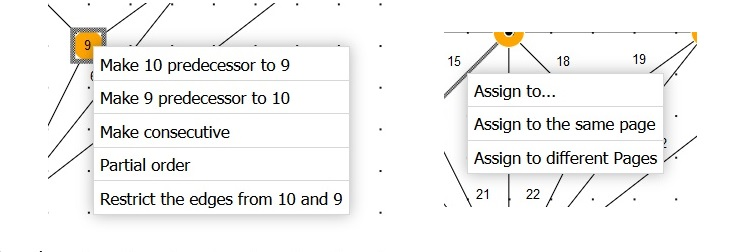
\includegraphics[width=\textwidth]{figures/figIndex/constraints.jpg}
\caption{Available constraints}
\label{img:constraints}
\end{center}
\end{figure}
\subsubsection{Restrict the linear order}
To restrict the linear order of the vertices, the user can impose the following constraints %(see Fig. \autoref{•}).
\begin{enumerate}
\item \textbf{Predecessor}
With this constraint the user can specify a relative order of the nodes by defining one node as the predecessor of another. It implicitly also provides successorship, by reversing the predecessor relation.
\item \textbf{Consecutivity} With this constraint two nodes can be required to be consecutive in the linear layout. It does not restrain the order of the nodes.
\item \textbf{Relative partial order} When selecting a sequence of at least two nodes an absolute partial order of these nodes can be either required or forbidden, meaning the exact order in which the nodes have been selected. If the nodes are not selected individually the order is determined by the time of creation.
\begin{figure}[!h]
\begin{center}

\includegraphics[width=1\textwidth]{figures/Platzhalter.png}
\caption{Platzhalter}
\label{img:plzhltr}
\end{center}
\end{figure}
\end{enumerate}
\subsubsection{Restrict the placement of edges}
\begin{enumerate}
\item \textbf{Assign edges to certain pages}
\textcolor{red}{Grafik}
By right clicking on a selection of at least one edge the user can assign these edges to pages of the linear layout. 
\item \textbf{Assign edges to the same page} Similar to assigning to certain pages, the user can also specify that the selected edges should be placed on the same page. 
\item \textbf{Assign edges to different pages}
As long as the user does not select more edges then there are pages available, the user can assure that all selected edges are on different half planes of the layout by using this constraint.
\item \textbf{Assign the edges incident to certain nodes}
\textcolor{red}{Grafik}
When the user rightclickes on two or more nodes, she can also constraint all edges incident to these nodes.\\
If exactly two vertices are selected, the user can also choose to only restrain the edges \textcolor{red}{how did this work again??}
\end{enumerate}
It is important to note that the corresponding constraints do only show up if the selection is exclusively nodes, respectively edges. Otherwise the context menu would be too unwieldy to use efficiently.
\section{Linear Layouts Viewer}
\subsection{Overview}
The viewer is structured similarly to the editing page, with a toolbar on top of the page, the viewing area in the middle and below a panel where user can change the appearance of the graph and see tthe constraits imposed on the graph.
\begin{figure}[!h]
\begin{center}

\includegraphics[width=1\textwidth]{figures/Platzhalter.png}
\caption{Overview 2}
\label{img:plzhltr}
\end{center}
\end{figure}
% how to transform graph, difficulty with arc edges, reading in constraints and pages etc, hash systems
\subsection{Linear layouts viewer}
% non editable but clickable
As a user accesses the second page, either directly or by redirection from the editor the site is checked for the hash parameter of the url. If it is not specified or not yet connected to a linear layout through the server, an error message shows up.\\
If the hash parameter is specified and \textcolor{red}{legit}, an ajax request is sent to the server.
The response is a javascript object literal and contains the following fields:
\begin{itemize}
\item id: the server id of the graph 
\item the graph: the 64 byte encoded graph that was sent to the server beforehand
\item pages: a list of javascript object literals, each object having an id property (the id of the page) as well as the type (stack or queue) and the layout (maximal, tree, forest, matching) of this page.
\item constraints: the constraints as javascript object literals, as they were sent to the server beforehand
\item status: either the string "IN\_QUEUE" or "READY". As long as the status is "IN\_QUEUE" all fields concerning the linear layout remain undefined.
\item assignments: a list of javascript object literals, each object having an edge property which contains the tag of an edge (string) and a page property containing the id of a page (string).
\item vertex order: a list strings, where each string is the tag of a vertex of the graph in the order the linear layout needs to be
\item satisfiability: a boolean stating whether the graph was embeddable as proposed
\item rawSolverResult: the output string of the lingeling SAT-solver
\item message: a potential error message, if the computation was not successful
\item created: a timestamp
\end{itemize}
After the website receives a response from the server it checks the status of the response. Should it be "IN\_QUEUE", another request is sent after 10 seconds. If the computation is finished the status is "READY".
Then as the second step the website checks if the graph is embeddable in the way it was defined, which is stated in the field \textit{embeddable}. If it is not embeddable a dialog shows up, allowing the user to go back to editing the graph.\\
If it is embeddable the website proceeds to modify the graph to display the linear layout in the following steps:
\begin{enumerate}
\item The graph is decoded and loaded into the viewer
\item The vertices are ordered according to the "vertex order" field of the responded embedding
\item The edges are divided into arrays representing each half plane of the graph, according to the "assignment" field\\
\item Each edge is assigned the "Arc Edge Style" provided by \textit{yFiles for HTML}. In order to display the edges correctly one extra step is needed: the position of each edge is determined by its source and target nodes, that is to say edges with a source node right to the target node are displayed beyond the nodes and when the source node is left to the target the edge is displayed above the nodes. As this would result in planes bearing the edges instead of half planes, the affected edges have to be found and have their source and targed swapped.
\item Each array representing one page of the linear embedding is assigned a color and placed alternatingly above and below the spine of the graph. 
\end{enumerate}
\subsection{Toolbar}
% mostly the same as before but less
\begin{figure}[!h]
\begin{center}

\includegraphics[width=1\textwidth]{figures/Platzhalter.png}
\caption{Toolbar 2}
\label{img:plzhltr}
\end{center}
\end{figure}
The toolbar of the second page is a thinned out version of the toolbar from the first page.\\
The \textbf{file} tab does no longer allow to load in graphMLs but still provides saving and exporting options.\\
The \textbf{view} tab still has the same options as before, being zooming in and out, fitting the graph on the page and toggeling the grid.\\
In addition to this it also provides the user with the option to examine the node neighborhood and edge adjacencies in the graph, as explained in section  \textcolor{red}{autoref -- ??}\\
The \textit{about} dialog can still be accessed on the second page and similar to the first page the user can hide the constraints panel at the bottom enlarge the graph viewing area. The \textit{stats} button is in the same place as before, too.\\
Instead of the \textit{compute} the toolbar contains a \textit{back to edit} button that takes the user back to the editor, with either the linear layout or the original layout as described in section \textcolor{red}{ autoref -- ??}\\
\subsubsection{Neighborhood and adjacency dialogs}
% neighborhood of a node, adjacency of an edge, necessary for analyzing
The \textit{node neighborhood} and the \textit{edge adjacency} buttons in the \textbf{view} tab of the toolbar, each open a dialog. \\
\begin{itemize}
\item The \textbf{node neighborhood} dialog holds information about the node that is currently selected and is only updated as a different, single node is selected. It lists the neighboring nodes and displays them in the color of the edge that connects the selected node to its neighbor.
\textcolor{red}{grafik}
\item The \textbf{edge adjacency} dialog tells the user what is the source and end node of the edge currently selected. Similar to the \textit{node neighborhood} it is only updated, when another edge is selected.
\end{itemize}
These dialogs proved to be useful to observe patterns in large embeddings, since following single edges turned out to be cumbersome.
\begin{figure}[!h]
\begin{center}

\includegraphics[width=1\textwidth]{figures/Platzhalter.png}
\caption{Neighborhood and Adjacency}
\label{img:plzhltr}
\end{center}
\end{figure}

\subsubsection{Returning to edit the graph}
By clicking on the "Return to edit" button in the upper right corner of the page, the user is redirected to the editing page. She or he may chose to either edit the original graph or the linear layout.\\
This functionality is obtained again by adding hash parameters to the redirection url. If the user choses to edit the original layout, the url gets extended by "\#or" and the id of the graph otherwise it is "\#ll" followed by the id. It proved useful because that way the user can not only be redirected to the original graph but also refer to the graph later on.\\
The editing page, recognizing if there is a hashparameter set, sends an ajax-request to the server similar to the viewing page. If the user wishes to edit the linear layout the same processes as described in \textcolor{red}{Ref} are triggered. When the original embedding is to be edited, each edge is also colored in the respective page color for easier observation but the graph is unchanged otherwise.\\
\begin{figure}[!h]
\begin{center}

\includegraphics[width=1\textwidth]{figures/Platzhalter.png}
\caption{Platzhalter}
\label{img:plzhltr}
\end{center}
\end{figure}
% displaying graph, hash system
\subsection{The something panel}
\subsubsection{Constraints}
In the bottom part of the page, the constraints defined in the creation of the graph are displayed in a similar fashion to the editing page, except that the user can not delete a constraint. \\
The constraints are stored in the server response as \textit{JavaScript} object literals. 

\subsubsection{Page representation}
The pages of the layout are again represented by a list of checkboxes. By unchecking pages their visibility can be toggled. Furthermore the representation of each page by selecting where to place the edges, either above or below the spine and by selecting a different color for the edges of a page. This is where the \textit{ColorPick}-plugin is used.
% visibility of edges, labels, color, colorpick etc
\begin{figure}[!h]
\begin{center}

\includegraphics[width=1\textwidth]{figures/Platzhalter.png}
\caption{Pages and Constraints Panel}
\label{img:plzhltr}
\end{center}
\end{figure}

\clearpage
